\documentclass[12pt]{article}
 
\usepackage[margin=1in]{geometry} 
\usepackage{amsmath,amsthm,amssymb}
\usepackage[lofdepth,lotdepth]{subfig}
\usepackage{graphicx}
\usepackage{float}
\usepackage{tikz}
\usetikzlibrary{arrows,shapes,trees} % loads some tikz extensions
 
\begin{document}
\graphicspath{{images/}}
 
\title{CSE 802 - Final Project Report\\ ImageNet Classification}
\author{Sunpreet Arora \& Josh Klontz\\
}
 
\maketitle

\section{Introduction}
Automated image classification is one of the classical problems in the domain of computer vision and pattern recognition. Although several algorithms exist for categorizing images based on their distinct characteristics or features, large scale image classification is still considered a significantly challenging task. This is primarily because it becomes difficult to find a sufficiently distinctive set of features to distinguish between large number of image classes. Besides, the computational complexity of the classification task scales up considerably as well.\\
The most common approach to image classification is based on the popular information retrieval model known as the bag-of-words (BOW) model. A \textit{visual vocabulary} is first created based on features computed from the training images. The frequency of occurrence of these features (also referred to as \textit{visual words}) in the visual vocabulary is then used for classifying images from the test set.\\
Several databases have been collected for advancing the state-of-the-art in image classification including Caltech 101 \cite{caltech101}, and PASCAL VOC \cite{pascal09}. ImageNet \cite{imagenet} is one of the most recent large scale image databases with 10,000 image classes, and over a million images. Convolutional neural networks (CNNs) have been reported to give the best rank-5 accuracy of around 85\% on the ImageNet database \cite{alex2012}. However, they were implemented on massive parallel GPU's. Another effective approach with a reported top-5 accuracy of 74\% involves Fisher vectors \cite{csurka2011fisher}.\\
The scope of this project however is limited to classifying a subset of 20 classes (10 hardest and 10 easiest) from the ImageNet database. We are given about 20000 images for training, 1000 images for validation and 5000 images for testing. The aim is to come up with a classification framework to maximize the rank-5 accuracy.

\section{Challenges}
Even though we are working with a subset of 20 distinct image classes from ImageNet, image classification is still very challenging. Some of the major challenging aspects are briefly discussed below:
\begin{enumerate}
\item \textit{Intraclass Variability}: Since ImageNet database is organized in a semantic hierarchy, exemplars from the same image class exhibit a considerable amount of variation or \textit{intraclass variability} amongst themselves. For example, both a gong and a wind chime belong to the semantic category (Figure \ref{fig1:subfig1}).
\item \textit{Interclass Similarity}: Similarly, exemplars from different classes such as spatula and ladle look visually similar to each other, or in other words exhibit \textit{interclass similarity} (Figure \ref{fig1:subfig2}).
\item \textit{Scale}: The object of interest is present at different scales in different exemplar images for each class (Figure \ref{fig1:subfig3}).
\item \textit{Pose}: Variations in pose of the object of interest are also observed amongst different exemplar images.
\item \textit{Illumination}: The database contains images acquired from a lot of different sources with differing illumination conditions.
\item \textit{Occlusion}: Sometimes the object of interest is occluded by another object in the image, thereby reducing the amount of useful information content for the classification task (Figure \ref{fig1:subfig4}).
\item \textit{Clutter}: There is a lot of background clutter in some of the exemplar images, or in other words there is more useless information present in the image than the useful one for the purpose of image classification.
\end{enumerate}

\begin{figure}
\centering
\subfloat[intraclass variability]{
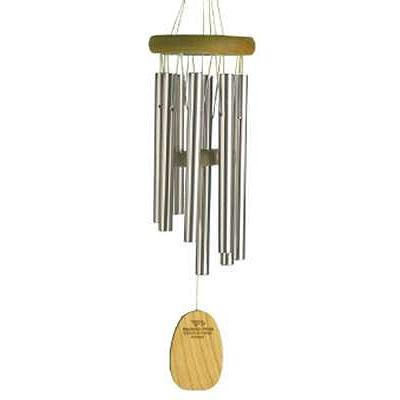
\includegraphics[width = 0.2\textwidth, height = 0.15\textheight]{chime1}
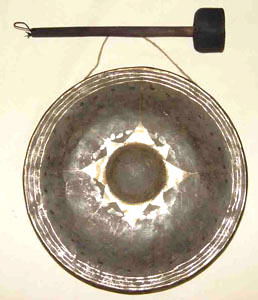
\includegraphics[width = 0.2\textwidth, height = 0.15\textheight]{chime2}
\label{fig1:subfig1}
}
\subfloat[interclass similarity]{
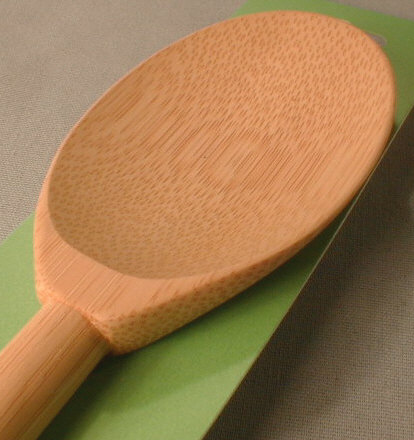
\includegraphics[width = 0.2\textwidth, height = 0.15\textheight]{spatula1}
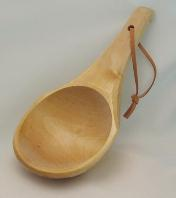
\includegraphics[width = 0.2\textwidth, height = 0.15\textheight]{ladle1}
\label{fig1:subfig2}
}
\qquad
\subfloat[scale]{
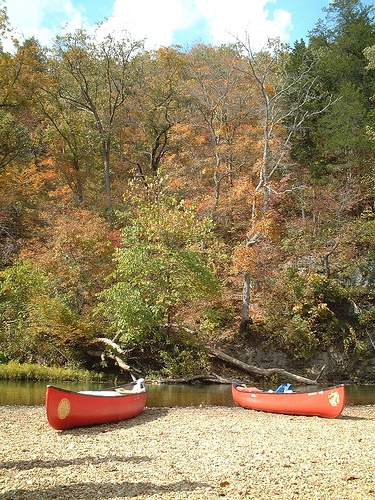
\includegraphics[width = 0.2\textwidth, height = 0.15\textheight]{canoe1}
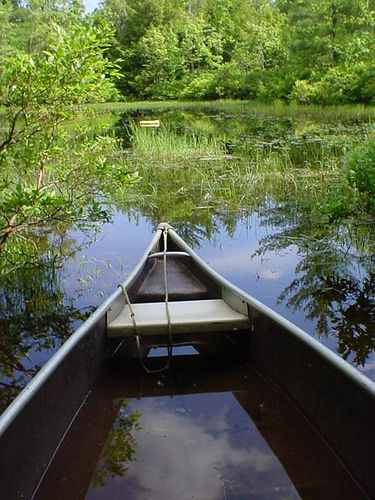
\includegraphics[width = 0.2\textwidth, height = 0.15\textheight]{canoe2}
\label{fig1:subfig3}
}
\subfloat[occlusion]{
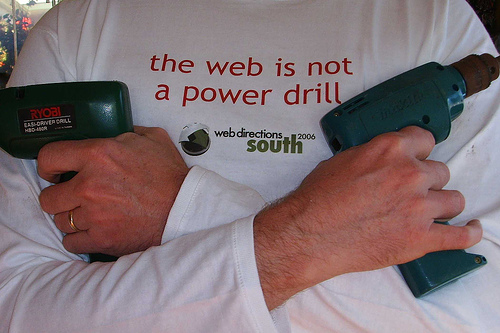
\includegraphics[width = 0.2\textwidth, height = 0.15\textheight]{pdrill1}
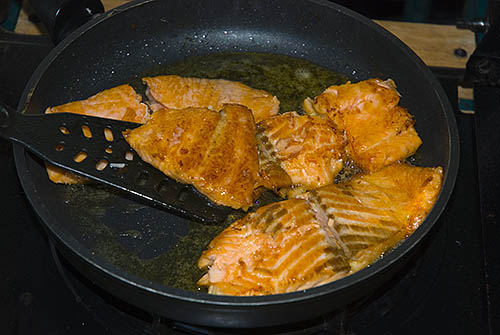
\includegraphics[width = 0.2\textwidth, height = 0.15\textheight]{spatula2}
\label{fig1:subfig4}
}
\caption{Some challenges in image classification}
\end{figure}

\begin{figure}
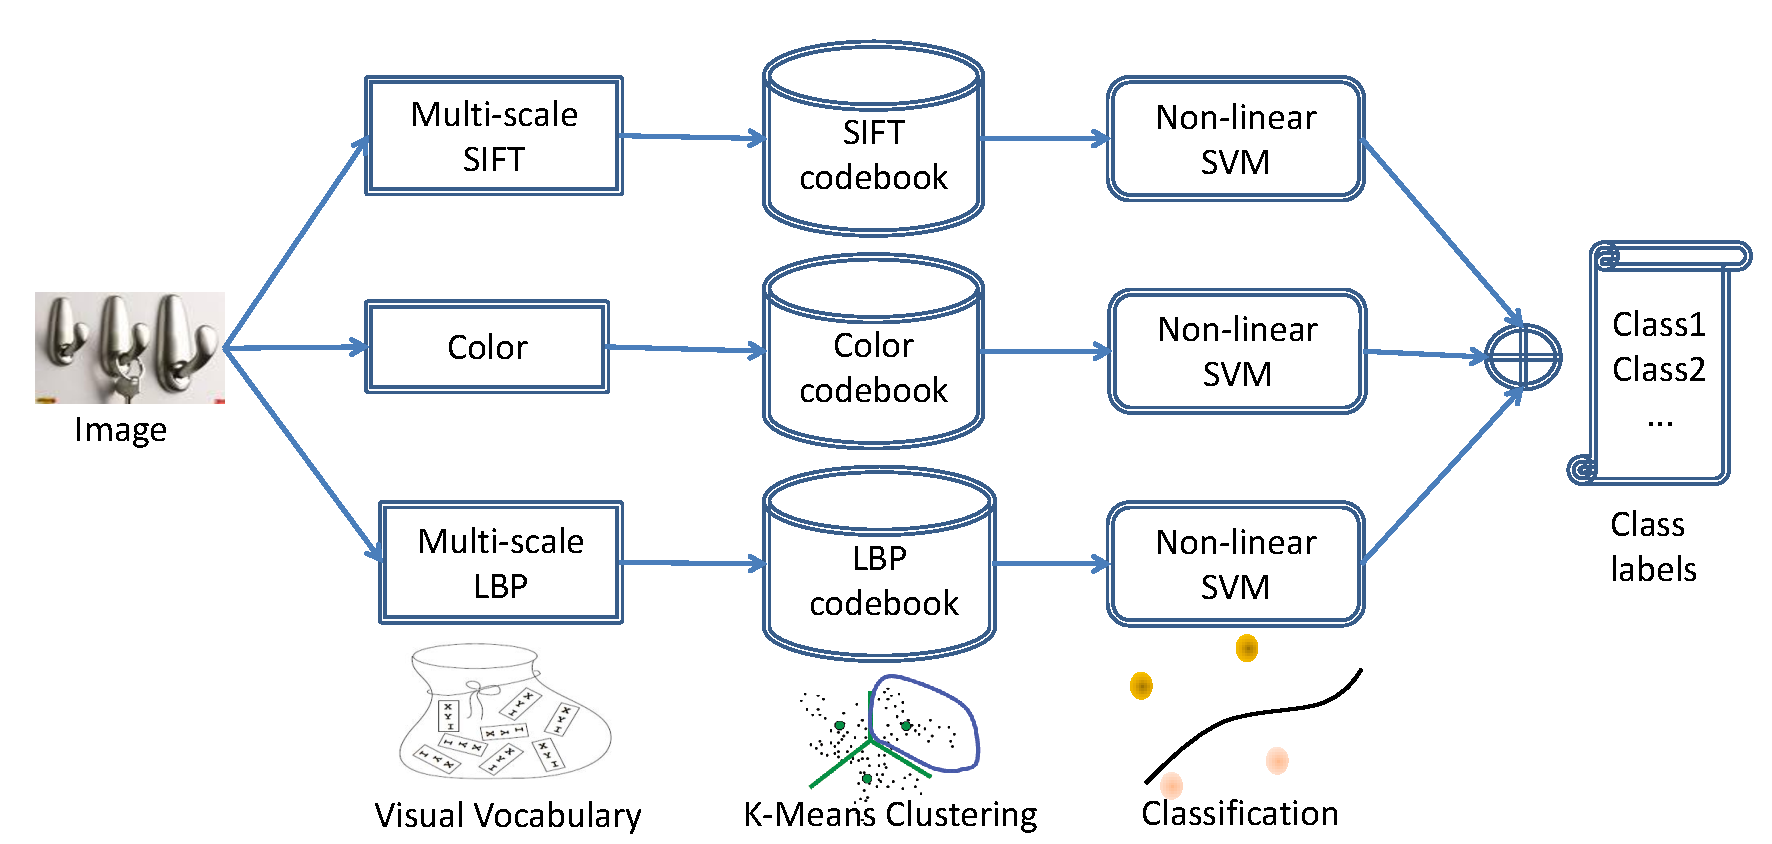
\includegraphics[width = 1\textwidth]{flowchart}
\caption{The proposed classification framework}
\end{figure}

\section{Framework}
For the given classification task, we propose a three stage framework based on the Bag of Words(BOW) model:
\begin{enumerate}
\item \textit{Multi-scale dense feature sampling for creating visual vocabulary}
\item \textit{K-means clustering for creating bag of words}
\item \textit{Non-linear support vector machines for classification}
\end{enumerate}

\bibliographystyle{plain}
\bibliography{report}

\end{document}